\section{Example}
\label{sec:example}

\begin{figure*}[t]
\centering
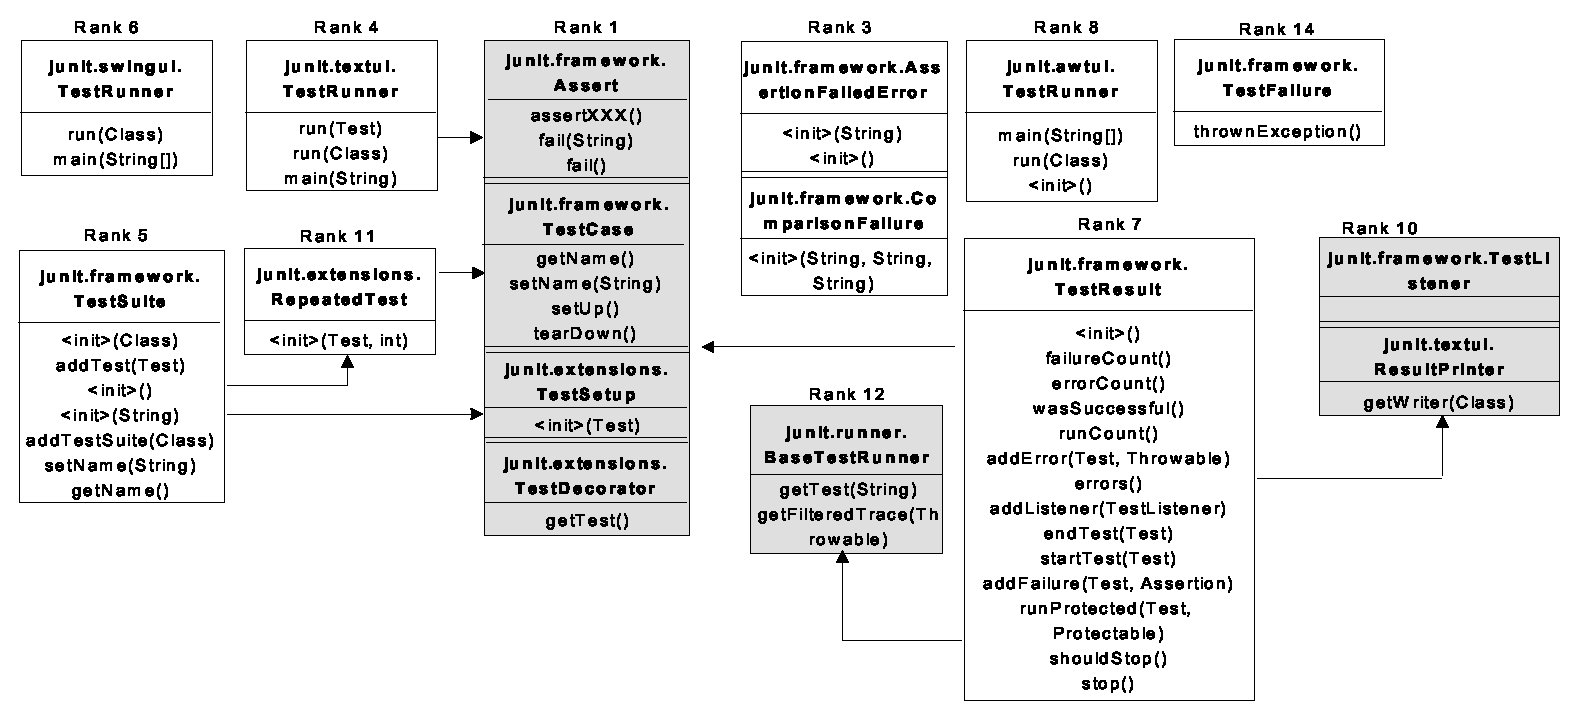
\includegraphics[scale=0.68,clip]{figs/examplehotspot_final.eps}
\caption{Hotspot hierarchies identified for the JUnit framework} \label{fig:hotspotexample}
\end{figure*}

We next use an example to explain our approach and show how the detected
hotspots and coldspots can be used by the framework users. We use JUnit~\cite{JUNIT}, the
\emph{de facto} standard unit testing framework for Java, 
as an illustrative example for explaining our approach.

SpotWeb accepts an input framework, say JUnit, and extracts
\emph{FrameworkInfo} from the framework. The
\emph{FrameworkInfo} includes all classes, all interfaces, public
or protected methods of each class and interface, and inheritance
hierarchy among classes or interfaces of the framework. SpotWeb also captures
the constants defined by the input framework. SpotWeb
constructs different queries for each class or interface and
interacts with a CSE such as Google code search~\cite{GCSE} to
gather relevant code examples from existing open source projects that
reuse the classes of the input framework. For example, SpotWeb constructs
a query such as ``\CodeIn{lang:java junit.framework.TestSuite}'' for
gathering relevant code examples of the \CodeIn{TestSuite} class. These
gathered code examples are referred as a \emph{LocalRepository} for
the input framework. SpotWeb analyzes gathered code examples
statically and computes \emph{UsageMetrics} for classes, interfaces,
and public or protected methods of all classes and interfaces. For
example, the \emph{UsageMetrics} computed for the \CodeIn{TestSuite}
class show that the class is instantiated for 165 times and is
extended for 32 times. Similarly, the \emph{UsageMetrics} computed
for the method \CodeIn{addTest} of the \CodeIn{TestSuite} class show
that the method is invoked for 95 times. SpotWeb also gathers code
examples for each class or method and stores these code examples in
a repository, referred as \emph{ExampleDB}. Then SpotWeb uses the
algorithm shown in Figure~\ref{alg:hotspotalgo} for detecting
hotspots from the computed \emph{UsageMetrics}.

Initially, SpotWeb ranks methods in a non-ascending order based on
their \emph{UsageMetrics} and uses a threshold percentage $HT$ to
detect hotspot methods: the methods in the top $HT$ percentage with
a non-zero \emph{UsageMetrics} are detected as hotspot methods. 
The detected hotspot methods are then
grouped into their declaring classes, detected as hotspot classes.
These hotspot classes are ranked based on the minimum rank of the
hotspot methods declared by these classes. SpotWeb classifies the
hotspot classes into two categories (templates and hooks) based on
heuristics described in Step 4 of the algorithm shown in Figure~\ref{alg:hotspotalgo}. The hotspot classes of each
category are further grouped into hierarchies based on their
inheritance relationships. For example, SpotWeb detected classes
\CodeIn{Assert} and \CodeIn{TestCase} as hook hotspots in the JUnit
framework. As \CodeIn{TestCase} class extends \CodeIn{Assert} class,
SpotWeb groups both the classes into the same hierarchy. SpotWeb
assigns a rank to each hierarchy based on the minimum rank of the
hotspot classes contained in the hierarchy. For example, consider
that the \CodeIn{Assert} class has Rank 1 and the \CodeIn{TestCase}
class has Rank 2, then the grouped hierarchy of the
\CodeIn{Assert} and \CodeIn{TestCase} classes is assigned with Rank
1. The rank attribute uniquely identifies a hierarchy among all
other hierarchies. Hierarchies with smaller ranks have higher preference
or importance to the hierarchies with larger ranks.

Figure~\ref{fig:hotspotexample} shows the hotspot hierarchies detected for the JUnit
framework. The figure also shows ranks assigned to each hierarchy.
As the rank attribute uniquely identifies a hierarchy, we use the
rank as an identity for describing a hierarchy.
Each hierarchy includes one or more hotspot classes and is shown as pairs of class and its methods.
For example, Hierarchy 1 (hierarchy with Rank 1) has classes \CodeIn{Assert}, \CodeIn{TestCase}, \CodeIn{TestSetup},
and \CodeIn{TestDecorator}. We show template hierarchies in white and hook hierarchies in gray.
For example, Hierarchy 1 is a hook hierarchy and Hierarchy 3 is a template hierarchy.

Methods inside each class of a hierarchy are sorted
based on their computed \emph{UsageMetrics}. Sorting methods of a class
can assist the framework users in quickly identifying the methods that are often
used inside a given hotspot class. For example, consider the \CodeIn{TestSuite} class
shown in Hierarchy 5. The \CodeIn{TestSuite} class has three constructors \CodeIn{<init>(Class)},
\CodeIn{<init>()}, and \CodeIn{<init>(String)}. However, the \CodeIn{<init>(Class)} constructor
is often used compared to the other two constructors. Due to space limit,
we show all assertion methods such as \CodeIn{assertEquals} and \CodeIn{assertTrue}
of the class \CodeIn{Assert} of Hierarchy 1 as \CodeIn{assertXXX}.

The figure also displays dependencies among hotspot hierarchies
(shown as arrows between hierarchies). SpotWeb captures the
usage relationships among hotspot classes through dependencies.
For example, Hierarchy $5$ has a
\CodeIn{TEMPLATE\_HOOK} dependency with Hierarchy $1$. This
dependency indicates that to reuse methods such as \CodeIn{addTest}
of the class \CodeIn{TestSuite} in Hierarchy 5, the user has to
define a new behavior for the classes in Hierarchy $1$.

\begin{figure}[t]
\begin{CodeOut}
\begin{alltt}
01:public class SRDAOTestCase 
02:\hspace*{0.4in}extends TestCase \{
03:\hspace*{0.1in}private SRDAO dao = null;...
04:\hspace*{0.1in}public SRDAOTestCase() \{
05:\hspace*{0.3in}super(); ... 
06:\hspace*{0.1in}\}
07:\hspace*{0.1in}protected void setUp() throws Exception \{
08:\hspace*{0.3in}...
09:\hspace*{0.3in}dao = (SRDAO)context.getBean("SRDAO");
10:\hspace*{0.3in}...
11:\hspace*{0.1in}\}
12:\hspace*{0.1in}public void tearDown() throws Exception \{
13:\hspace*{0.3in}dao = null; 
14:\hspace*{0.1in}\}
15:\hspace*{0.1in}public void testF() \{ ... \}
16:\hspace*{0.1in}public void testB() \{ ... \}
17:\hspace*{0.1in}...
18:\}
\end{alltt}
\end{CodeOut}
\Caption{\label{fig:hcodeexample} Suggested code example for the hook class \CodeIn{TestCase}.}
\begin{CodeOut}
\begin{alltt}
01:public class MyTestSuite \{ 
02:\hspace*{0.1in}...
03:\hspace*{0.1in}public static Test suite() \{
04:\hspace*{0.3in}TestSuite suite = new TestSuite("axis");
05:\hspace*{0.3in}suite.addTest(new SRDAOTestCase());
06:\hspace*{0.3in}return suite;
07:\hspace*{0.1in}\}
08:\hspace*{0.1in}...
09:\}
\end{alltt}
\end{CodeOut}
\Caption{\label{fig:tcodeexample} Suggested code example for the template class \CodeIn{TestSuite}.}
\end{figure}

We next describe how the hotspots detected by SpotWeb can be used by
the framework users to reuse classes of the JUnit framework. After reviewing
the hotspots shown in Figure~\ref{fig:hotspotexample}, consider that
a framework user wants to start with the method \CodeIn{addTest} of
the template class \CodeIn{TestSuite} in Hierarchy 5.
Figure~\ref{fig:hotspotexample} shows that Hierarchy 5 of the
\CodeIn{TestSuite} class has a \CodeIn{TEMPLATE\_HOOK} dependency
with the Hierarchy 1. This dependency indicates that the user may
need to define a new behavior for the associated hook hierarchy.
SpotWeb recommends the code example shown in
Figure~\ref{fig:hcodeexample} for the hook class \CodeIn{TestCase},
which is part of Hierarchy 1. The code example exhibits several
aspects that need to be handled by the user while extending the
\CodeIn{TestCase} class. For example, in the \CodeIn{setUp} method,
the user can write code for setting up the environment such as
instantiating necessary variables, and in the \CodeIn{tearDown}
method, the user can destroy the created variables. In addition, the code
example shows that names of the test methods in the extended class
of the \CodeIn{TestCase} class should start with the prefix \CodeIn{test}.
SpotWeb also recommends a code example for the \CodeIn{addTest} method and
the recommended code example is shown in
Figure~\ref{fig:tcodeexample}. The code example shows that the user
has to create an instance of the \CodeIn{TestSuite} class and then
add test cases through the \CodeIn{addTest} method.

An API class or method is identified as a coldspot if that class or method is neither
used directly nor used indirectly by gathered code examples. The complete
algorithm used for detecting coldspots is shown in Figure~\ref{alg:coldspotalg}. SpotWeb identified $20$
classes such as \CodeIn{Swapper}, \CodeIn{TestRunListener}, and \CodeIn{ExceptionTestCase} as coldspots
in the JUnit framework. However, coldspots are only suggestions
for users unfamiliar to that framework and SpotWeb does not intend to recommend users not to reuse
those coldspot classes. Sometimes, coldspots can also be helpful to
the framework developers in distributing their maintenance efforts, because the framework
developers can give a low preference to the coldspot classes.
